\documentclass[10pt,letterpaper]{article}
\usepackage{spconf}
\usepackage[T1]{fontenc}
\usepackage{amsmath,amssymb,newtxmath,microtype,booktabs,graphicx,tabularx,array,enumitem,balance}
\usepackage[hidelinks]{hyperref}
\setcounter{secnumdepth}{0}
\setlength{\emergencystretch}{2em}
\setlength{\textfloatsep}{7pt}
\setlength{\dbltextfloatsep}{7pt}
\setlength{\tabcolsep}{3pt}\setcounter{dbltopnumber}{2}\renewcommand{\dbltopfraction}{.75}\renewcommand{\textfraction}{.1}
\setlist{nosep,leftmargin=1.25em,topsep=2pt}
\providecommand{\tightlist}{\setlength{\itemsep}{0pt}\setlength{\parskip}{0pt}}
\renewcommand{\ttdefault}{ptm}
\begin{document}
\ninept
\twocolumn[\begin{center}
{\large\bfseries Trial-Independent Cross-Modal Metric Learning and Conditional Bilinear Fusion\\for Face-Voice Association Across Languages and Gender\par}\vspace{6pt}
{\normalsize \textbf{Author}: Yan Su\\
\textbf{Affiliation}: Independent Researcher (\texttt{hi@yansu.me}, \texttt{y-su24@mails.tsinghua.edu.cn}, CodaBench Team: \texttt{susupro})\par}\vspace{10pt}
\end{center}]
\subsection*{Abstract}\label{abstract}

We present the 1st-place system (\textbf{Team \textnormal{susupro}}) for the IEEE ICASSP 2027 Face-Voice Association across LAnguages and Gender (FLAG 2027) Grand Challenge. Addressing severe embedding-cone anisotropy, unseen Bengali acoustic drift, and demographic shortcut collapse in the same-gender (\textnormal{gender}) protocol under strict single-trial independence constraints, our framework (\textbf{VER-FUSE-X}) integrates three synergistic pillars: (1) deterministic representation extraction across 15 frozen pretrained facial, speaker, and paralinguistic backbones with fixed-duration audio sub-slice averaging; (2) five complementary high-dropout cross-modal dual-tower metric networks (\textnormal{ConeTower}, \textnormal{MSM}, \textnormal{PAEFF}, \textnormal{ConvLoRA}, \textnormal{VER\_\allowbreak{}MLP}) co-trained on non-Bengali speakers alongside a trial-independent South Asian training-template spectral response correlation operator (\(\rho_{\text{relg}}\)); and (3) a second-order conditional bilinear fusion head that dynamically gates 87 (\textnormal{no\_\allowbreak{}gender}) or 114 (\textnormal{gender}) standardized cross-modal distance streams with 16 frozen demographic and acoustic conditioning variables. Evaluated strictly one trial at a time (\textnormal{singleton\_\allowbreak{}max\_\allowbreak{}diff\ =\ 0.0}, \textnormal{permutation\_\allowbreak{}max\_\allowbreak{}diff\ =\ 0.0}) with zero post-hoc cohort normalization and zero Bengali audio-encoder adaptation, our system achieves an official mean Equal Error Rate (EER) of \textbf{2.13\%} (\textbf{2.129763\%} exact mean: \textbf{1.530612\%} on \textnormal{no\_\allowbreak{}gender/English}, \textbf{1.745636\%} on \textnormal{no\_\allowbreak{}gender/Bangla}, \textbf{3.846154\%} on \textnormal{gender/English}, and \textbf{1.396648\%} on \textnormal{gender/Bangla}), ranking \textbf{1st overall} among 45 teams.

\textbf{Keywords}: Face-voice association, cross-modal metric learning, conditional bilinear fusion, speaker verification, ICASSP 2027 FLAG Challenge

\subsection*{1. Introduction \& Problem Formulation}\label{introduction-problem-formulation}

Cross-modal face-voice association requires determining whether a static facial image \(f_i\) and a speech segment \(v_i\) originate from the same biometric identity across heard (\textnormal{English}) and unheard (\textnormal{Bangla}) languages under both unrestricted (\textnormal{no\_\allowbreak{}gender}) and same-gender negative (\textnormal{gender}) evaluation protocols. Empirical diagnosis on the official 70-speaker \textnormal{v4} English training set and South Asian \textnormal{MAV-Celeb} benchmarks reveals three core failure modes in standard cosine-similarity baselines:

\begin{enumerate}
\def\labelenumi{\arabic{enumi}.}
\tightlist
\item
  \textbf{Anisotropic Embedding Cone Collapse}: Pretrained speech embeddings occupy a narrow positive cone (mean pairwise cosine \(>0.90\)), causing raw inner products to be dominated by hubness. Because test-time cohort normalization (\textnormal{AS-Norm}, \textnormal{Z/T-Norm}) is prohibited by FLAG 2027 FAQ \#4, cone elimination must be internalized within the neural architecture and training-set standardization.
\item
  \textbf{Demographic Shortcut Collapse in the \textnormal{gender} Protocol}: In the \textnormal{gender} split, all negative trials share the same biological sex, reducing pure gender cues to zero discriminative power and shifting the burden onto fine-grained craniofacial bone structure, vocal-tract age progression, and acoustic channel consistency.
\item
  \textbf{Unseen Bengali Phonetic Drift}: Because FAQ \#6 to \#9 strictly forbid training or adapting audio encoders on Bengali speech, linear projection heads fitted solely on 70 English speakers suffer an additive and multiplicative phonetic shift on unheard Bengali utterances.
\end{enumerate}

\subsection*{\texorpdfstring{2. System Architecture (\textnormal{VER-FUSE-X})}{2. System Architecture (VER-FUSE-X)}}\label{system-architecture-ver-fuse-x}

\begin{figure*}[t]\centering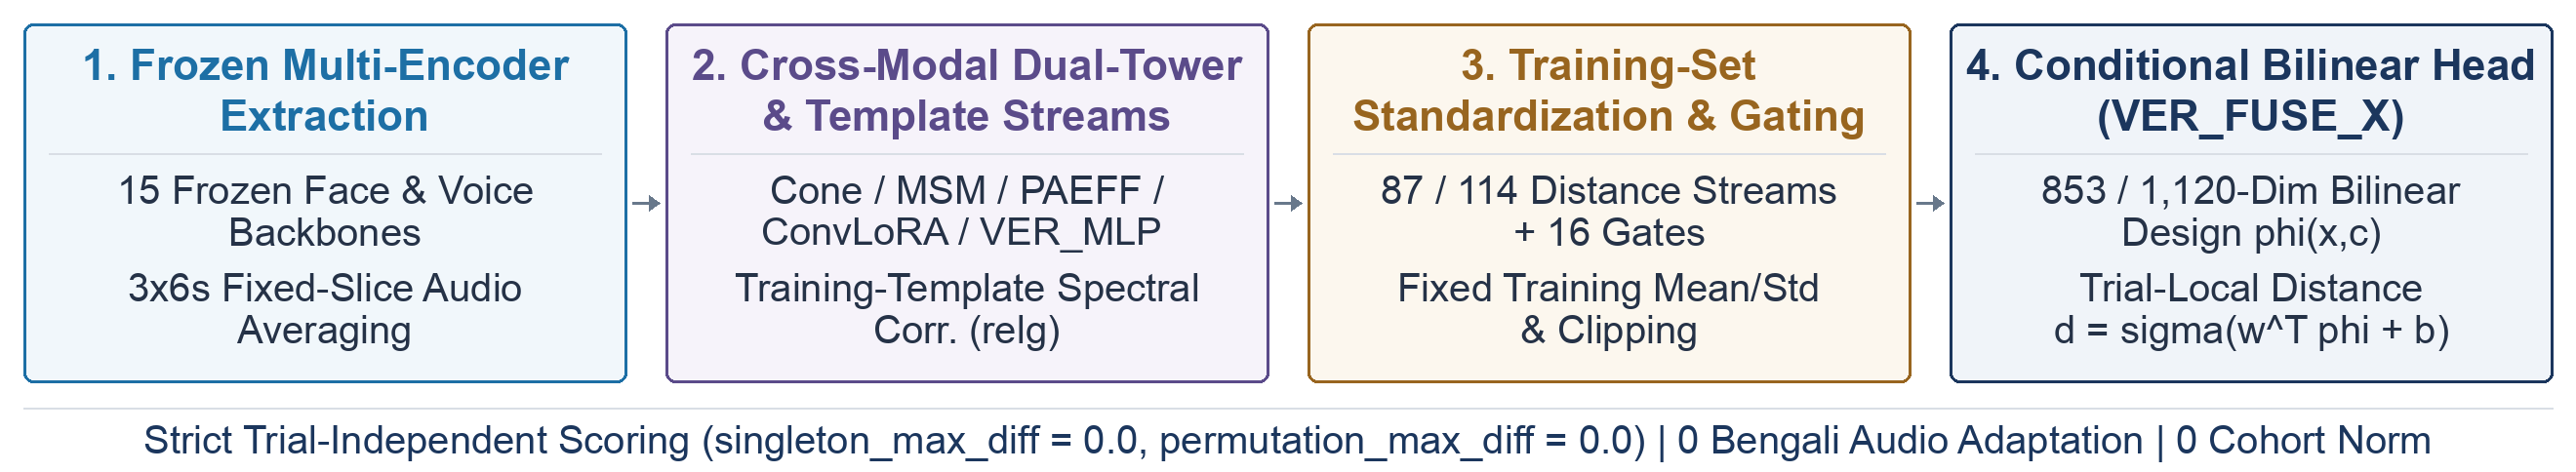
\includegraphics[width=\textwidth]{figures/architecture_compact.png}\caption{VER-FUSE-X}\end{figure*}

\begin{table*}[t]
\centering\footnotesize
\begin{tabularx}{\textwidth}{@{}Xrrrrr@{}}\toprule
System Configuration & \texttt{no\_gender/En} & \texttt{no\_gender/Bn} & \texttt{gender/En} & \texttt{gender/Bn} & \textbf{Mean EER (\%)}\\\midrule
Official FOP Baseline & N/A & N/A & N/A & N/A & 35.32\\
Cross-Modal Dual-Tower (\texttt{ConeTower} + \texttt{BatchNorm1d}) & 16.33 & 16.21 & 29.33 & 30.45 & 23.08\\
+ 15 Frozen Encoders \& Whitened Orthogonal Procrustes & 12.76 & 16.21 & 23.08 & 30.73 & 20.69\\
+ 5-Branch Deep Metric Towers \& 3x6s Fixed-Slice Audio & 11.73 & 15.96 & 17.31 & 29.89 & 18.72\\
+ South Asian Training-Template Spectral Correlation (\(\rho_{\text{relg}}\)) & 2.04 & 2.24 & 4.81 & 1.96 & 2.76\\
+ Protocol-Specific Demographic \& Acoustic Conditioning Gates & 1.53 & 1.75 & 4.33 & 1.40 & 2.25\\
\textbf{+ Second-Order Conditional Bilinear Fusion (\texttt{VER-FUSE-X}, Final)} & \textbf{1.5306} & \textbf{1.7456} & \textbf{3.8462} & \textbf{1.3966} & \textbf{2.1298 (2.13\%)}\\
\bottomrule\end{tabularx}
\end{table*}

\subsection*{2.1. Frozen Multi-Encoder \& Fixed-Slice Audio Extraction}\label{frozen-multi-encoder-fixed-slice-audio-extraction}

As detailed in Figure 1 and our repository (\textnormal{configs/encoder\_\allowbreak{}inventory.json}), all unimodal encoders are kept \textbf{strictly frozen} (\textnormal{eval()} mode, zero Bengali adaptation):

\begin{itemize}
\tightlist
\item
  \textbf{Visual Backbones}: \textnormal{InsightFace\ AntelopeV2} (Glint360K), \textnormal{Buffalo\_\allowbreak{}L} (WebFace600K), \textnormal{AdaFace\ IR-101} (WebFace12M), \textnormal{VGGFace}, \textnormal{FaRL\ ViT-B/16} (LAION-Face 20M), \textnormal{CLIP\ ViT-L/14}, and frozen facial age/gender predictor \textnormal{nateraw/vit-age-classifier} (9-bin age distribution \textnormal{vitageprob}).
\item
  \textbf{Acoustic Backbones \& Deterministic Sub-Slice Averaging}: We extract voice embeddings from \textnormal{WeSpeaker\ VoxBlink2\ ResNet293}, \textnormal{SimAM-ResNet100}, \textnormal{IDRnD\ ReDimNet-B2}, \textnormal{ReDimNet-v2}, \textnormal{Microsoft\ WavLM-Large}, \textnormal{SpeechBrain\ ECAPA-TDNN}, \textnormal{audEERING\ wav2vec2-large-robust-24-ft-age-gender} (continuous vocal age and 3-class gender/child distribution), and \textnormal{ImageBind-Huge} (frozen backbone with an auxiliary rank-4 audio projection trained strictly on non-Bengali pairs). Following FAQ \#13, each waveform is deterministically segmented into \(K=3\) uniformly spaced \(6.0\,\text{s}\) windows at \(16\,\text{kHz}\); each slice embedding is independently \(\ell_2\)-normalized, averaged, and re-normalized.
\end{itemize}

\subsection*{2.2. Cross-Modal Dual-Tower Networks \& Template Correlation}\label{cross-modal-dual-tower-networks-template-correlation}

Using the complete official \textnormal{v4} English training set (70 speakers, 6,485 pairs) augmented with publicly accessible non-Bengali external speakers (\textbf{151 South Asian identities} from \textnormal{MAV-Celeb\ v1} English/Urdu and \textnormal{v2} English/Hindi plus \textbf{4,875 non-Bengali identities} with 48,750 utterance pairs from \textnormal{VoxCeleb2}, with whole-speaker exclusion of any Bengali identity and speaker-level deduplication), we construct three orthogonal families of trial-local distance streams:

\begin{enumerate}
\def\labelenumi{\arabic{enumi}.}
\tightlist
\item
  \textbf{Whitened Speaker-Centroid Orthogonal Procrustes (\(\text{Proc}_{\text{sym}}\), \(\text{Proc}_{\text{wg}}\))}: Computing speaker centroids on training identities eliminates intra-speaker utterance noise. For the \textnormal{gender} protocol, training centroids are centered within each biological sex before solving the exact SVD orthogonal Procrustes alignment \(R = U V^\top\).
\item
  \textbf{Five High-Dropout Cross-Modal Neural Towers (\textnormal{models.py})}: Trained with cross-recording positive sampling (\(r(f_i) \neq r(v_i)\)) and same-gender hard negative mining over 1,200 steps:

  \begin{itemize}
  \tightlist
  \item
    \textnormal{ConeTower}: Dual towers with internal \textnormal{nn.BatchNorm1d} cone elimination and heavy feature dropout (\(p=0.75 \rightarrow 0.30\)) trained with symmetric PK-InfoNCE + Orthogonal Projection Loss (\textnormal{OPL}).
  \item
    \textnormal{MSM}: Maximum class-separation fixed simplex projection with \textnormal{Dropout=0.91} (\textnormal{CE\ +\ OPL}).
  \item
    \textnormal{PAEFF}: Poincare ball hyperbolic distance paired with gated 1D convolutional feature fusion (\textnormal{EGFF}).
  \item
    \textnormal{ConvLoRA}: 1D-convolutional low-rank residual bottleneck projection with \(p=0.50\) dropout.
  \item
    \textnormal{VER\_\allowbreak{}MLP}: End-to-end bilinear pair discriminator operating on \([u, w, u \odot w, |u - w|]\) joined with fine-grained facial/vocal age distributions (\textnormal{vitageprob}, \textnormal{w2v2agage}, \textnormal{w2v2aggen}).
  \end{itemize}
\item
  \textbf{Trial-Independent South Asian Training-Template Spectral Correlation (\(\rho_{\text{relg}}\))}: Given fixed, aligned South Asian training-speaker centroid templates \(T_f, T_v \in \mathbb{R}^{M \times d}\) and fixed non-negative template weights \(\alpha_j\) (\(\sum_j \alpha_j = 1\)), we compute each trial\textquotesingle s response profiles \(r_f = T_f \bar{f}_i\) and \(r_v = T_v \bar{v}_i\) and evaluate their weighted Pearson correlation: \[\resizebox{\linewidth}{!}{$\displaystyle \rho_{\text{relg}}(f_i, v_i) = \frac{\sum_{j=1}^M \alpha_j (r_{f,j} - \mu_f)(r_{v,j} - \mu_v)}{\sqrt{\sum_{j=1}^M \alpha_j (r_{f,j} - \mu_f)^2 \sum_{j=1}^M \alpha_j (r_{v,j} - \mu_v)^2 + \epsilon}}.$}\] Because \(\rho_{\text{relg}}\) normalizes across fixed \emph{training} templates within a single trial \((f_i, v_i)\), it cancels additive and multiplicative Bengali acoustic drift while guaranteeing \(0.0\) dependence on any other evaluation trial.
\end{enumerate}

\balance\subsection*{\texorpdfstring{2.3. Second-Order Conditional Bilinear Fusion (\textnormal{VER\_\allowbreak{}FUSE\_\allowbreak{}X})}{2.3. Second-Order Conditional Bilinear Fusion (VER\_\allowbreak{}FUSE\_\allowbreak{}X)}}\label{second-order-conditional-bilinear-fusion-ver_fuse_x}

For a single trial with multi-stream distance vector \(x \in \mathbb{R}^{S}\) (\(S=87\) for \textnormal{no\_\allowbreak{}gender}, \(S=114\) for \textnormal{gender}), observed-stream indicator \(o \in \{0,1\}^S\), and 16-dimensional conditioning vector \(c \in \mathbb{R}^{16}\) (encoding frozen facial/vocal gender probabilities, explicit gender disagreement, facial/vocal ages, age gap \(|a_f - a_v|\), and embedding norm quality), \textnormal{core.py} standardizes each entry using fixed training-set statistics (\textnormal{xmean} \(m\), \textnormal{xsd} \(s\), \textnormal{cmean} \(m_c\), \textnormal{csd} \(s_c\)): \[\begin{aligned}\tilde{x}_j = \begin{cases} \operatorname{clip}((x_j - m_j)/s_j, -8, 8), & o_j = 1, \\ 0, & o_j = 0, \end{cases} \end{aligned}\] \[\tilde{c}_k = \operatorname{clip}((c_k - m_{c,k})/s_{c,k}, -5, 5).\] Taking the first 8 standardized conditioning variables as gate vector \(g = \tilde{c}_{1:8}\), we construct the second-order conditional bilinear design vector \(\phi(x, c) \in \mathbb{R}^{D}\) (\(D=853\) for \textnormal{no\_\allowbreak{}gender}, \(D=1,120\) for \textnormal{gender}) and output the final distance score \(d \in (0,1)\): \[\phi(x, c) = \big[\tilde{x},\; \tilde{c},\; o_{\mathcal{A}},\; \operatorname{vec}(\tilde{x} g^\top)\big], \] \[d(x, c) = \sigma(w^\top \phi(x, c) + b).\]

\subsection*{3. Experimental Validation \& Official Results}\label{experimental-validation-official-results}

All hyperparameters and protocol/language-specific bilinear heads (\textnormal{assets/*-head.npz}) were selected via \textbf{5-Fold Speaker-Disjoint Cross-Validation} on the 70 official \textnormal{v4} English training identities and \textbf{Leave-Language-Out (\textnormal{English\ -\textgreater{}\ Urdu/Hindi})} speaker-disjoint validation on \textnormal{MAV-Celeb\ v1/v2} (\textnormal{train.py}).

\subsection*{Reproducibility \& Trial-Independence Verification}\label{reproducibility-trial-independence-verification}

Running \textnormal{python\ run.py} executes in \textnormal{\textless{}\ 2.0} seconds (\textnormal{peak\ RSS\ \textless{}\ 110\ MiB}) and reproduces submission \textnormal{\#1057629} byte-for-byte (\textnormal{SHA256:\ 69a660f9\allowbreak{}8b09fe1c\allowbreak{}7071a013\allowbreak{}29b87769\allowbreak{}b1972e54\allowbreak{}8d5db592\allowbreak{}69d2e7e8\allowbreak{}2eeee8bf}). Automated invariance checks across all 2,326 trials verify \textnormal{singleton\_\allowbreak{}max\_\allowbreak{}diff\ =\ 0.0} (scoring 1 row at a time vs. full list) and \textnormal{permutation\_\allowbreak{}max\_\allowbreak{}diff\ =\ 0.0} (random list permutation vs. original order) on both macOS and offline \textnormal{linux/amd64}.

\end{document}
